\begin{figure}[h]
	\centering
	
\includegraphics[scale=.20]{applogo}
	\caption{Google App Engine Logo}
	\label{Fig:applogo}	
\end{figure}

Google App Engine is a Platform as a Service (\textit{PaaS}) which allows users to build and run web applications on Google  infrastructure.

Thus, when a programmer writes a web application that runs on App Engine, the software is going to run on the Google servers, somewhere in the Google cloude \cite{UGAE}. This solution is very useful because allows everyone to write the own web program without purchasing and maintaining the needed hardware and network.

For the time being Google App Engine supports web applications written in a variety of the main programming languages for the web: \textit{Java}, \textit{Python}, \textit{PHP}, and \textit{GO}. Since the App Engine was first built in $2008$ for Python, this is the language used to carry out the web application for this thesis.

Over the possibility to create our own web application without dealing with hardware, the Google App Engine has been chosen because of its datastore and memcache, which allow a simple memorization of data, automatic scaling and load balancing, and more others important features that are going to be shown below.

To create a more scalable and hierarchical web application the \textit{Flask framework} has been used. Flask is a lightweight web application framework written in Python. It is based on the \textit{WSGI} toolkit and Jinja2 template engine and it is distributed with a \textit{BSD} license.\\ Flask provides an easy way to organize a web application which allows to build up complex website easy to manage. It has no database abstraction layer, indeed for this purpose, in this application, it supports the Google App Engine.

\begin{figure}[h]
	\centering
	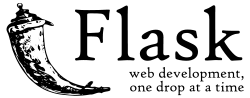
\includegraphics[scale=.8]{flask}
	\caption{Flask Logo}
	\label{Fig:flasklogo}	
\end{figure}

Before to explain how the code is made, the App Engine Datastore and Memcache are going to be introduced.\\
Using  the Google App Engine means do not have access to traditional database like Oracle and MySQL. In fact, App Engine uses \textit{\textbf{Google Datastore}}, which is easier to use because it takes more of a hierarchical object-oriented storage approach. That approach allows to ensure efficient application scalability.
Thus, the Datastore holds data objects known as \textit{entities}. An entity is composed by one or more \textit{properties}. Making a comparison with the object oriented it is possible to say that the properties are the fields of objects. So, likely the field, a property may support different data types such as integer, float, string and so on... Any entity holds its \textit{kind} and \textit{key}, which categorize and uniquely identify it, respectively. 

The \textit{memcache} results very useful to speed up common Datastore queries, indeed inside the Google Datastore, distributed memory cache are used for storage.
For this reason memcache is used to store the status of the electrovalves, in fact in this way the delay caused by the server is highly reduced.

\section{The web application}

The main code which runs on server is shown in (List.\ref{code:server}). It uses two models to describe the data supposed to be stored:
\begin{enumerate}
	\item \textit{Sensor}, contains the list of sensors used from the system, through the method \textit{sensor\_list} it returns that list;
	\item \textit{DataPoint}, contains all the points that have to be plotted, the field value represent the $y-axes$ while time the $x-axes$. While the first field has to be passed at the moment in which the class is constructed, the \textit{date} field is auto-filled with the current data. This class has two public methods to interact with: 
	\begin{itemize}
		\item \textit{point\_for\_sensor}, that with the name of sensor as parameter returns the list of \textit{DataPoint} associated;
		\item \textit{oldest\_point}, that returns the last \textit{DataPoint} inserted.
	\end{itemize} 
 \end{enumerate} 
 
 Below the different services offered by this web application are listed:
 \begin{itemize}
 	\item \textit{process\_values}, available at the path \url{/sensor_values}. User can access to this service using both \textit{HTTP} \textit{GET} and \textit{POST} methods. With the first one, it  returns the \textit{JSON} (\textit{JavaScript Object Notation}) containing all the data regarding the whole sensors stored inside the Datastore, in this format: \{ value, timestamp, sensor\_name \}. On the other hand, when the used method is \textit{POST} the application takes from the POST parameters those named \textit{"sensor"}, indicating the sensor's name, and \textit{"value"}, which is the sensor's value that has to be plotted. Thus, in this last way what the application does is to add a new data point for a sensor and store it inside the Datastore.
 	\item \textit{print\_names}, available at the path \url{/sensor_names}. This function is accessible only through HTTP \textit{GET} method and returns a \textit{JSON} object with the content of sensor's name list.
 	\item \textit{graphing\_data}, available at the path \url{/graphing_data}. To access to  this function a HTTP \textit{GET} method is required. This \textit{GET} request must contain two parameters: \textit{"sensor"}, the sensor name, and \textit{"first\_timestamp"}, which is the timestamp of the first point that has to be plotted. This last parameter is not mandatory and if it is missed it is assumed equal to $0$. What this function does is to return a \textit{JSON} object containing the whole DataPoint for the given sensor that have timestamp higher than \textit{"first\_timestamp"}.
 	\item \textit{clear\_data}, available at the path \url{/clear}. This function is in charge to deletes all the points for each sensor.
 	\item \textit{set\_picture}, available at path \url{/picture/submit}. This function is accessible with both HTTP \textit{POST} and \textit{GET} methods, and in both cases its behavior is to load a new image, containing the beating plot, onto Datastore. In the first case the image has be passed ad \textit{POST} data, and named as \textit{"Image.jpg"}. While th second case is supposed to be a browser way to upload the image. In fact, browsing to that \textit{URL} what the user sees is shown in (Fig.\ref{Fig:http}), a view where it is possible to select the picture file and submit it.
 	
 	\begin{figure}[h]
 		\centering
 		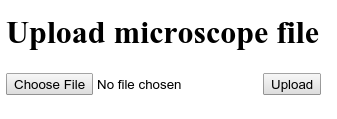
\includegraphics[scale=.8]{http}
 		\caption{Picture Submitting from the Browser}
 		\label{Fig:http}	
 	\end{figure}
 	
 	\item \textit{view\_picture}, available at the path \url{/picture/view}. Using this function, with a HTTP \textit{GET} method causes the access to the image previously stored inside the Datastore.
 	\item \textit{set\_video}, available at the path \url{/video/submit}. As happened to the beating plot image, this function is accessible with both HTTP \textit{POST} and \textit{GET} methods. And, as before, it is used to load onto Datastore the microscope video. Using the \textit{POST} method means storing the data passed as parameter and named \textit{"Video.mp4"}. On the other hand, in case of GET method what the user sees on the browser is shown in (Fig.\ref{Fig:http1}). As before, through the two buttons, user can choose the video to store and submit the request.
 	
 	\begin{figure}[h]
 		\centering
 		
\includegraphics[scale=.8]{http1}
 		\caption{Video Submitting from the Browser}
 		\label{Fig:http1}	
 	\end{figure}
 	
 	\item \textit{view\_video}, available at the path \url{/video/view}. This function, accessible with HTTP \textit{GET} method, accesses to the microscope's video on the Datastore and returns it.
 	
 	\item  \textit{add\_electrovalve}, available at the path \url{/add/electrovalve}. This function is in charge to store the valve's status inside the memcache. It is accessible through HTTP \textit{POST} method, which must have these two following parameters:\textit{ "name"}, that uniquely identifies the valves (it is \textit{"EV"} follows by the number of the valve, for example the first one is \textit{"EV1"}), and \textit{"status"}, which indicates the actual status of the valve (it may be \textit{on} or \textit{off}).
 	
 	\item \textit{get\_electrovalve}, available at the path \url{/electrovalves/<name>}. It is accessible through HTTP \textit{GET} method and returns the value of the valve identified with \textit{<name>} field inside the \textit{URL} (for example, if someone wants to read the status of the first valve, has to use the path \url{/electrovalves/EV1}).
 	
 	
 	
 \end{itemize}
 